% =============================================================================
%  RahiScan: Automated Rickshaw Fare & Pace Telemetry
%  Introduction to Data Science - Case-Study Proposal
%  Compile with XeLaTeX or Tectonic:   tectonic RahiScan_Proposal.tex
% =============================================================================
\documentclass[12pt, a4paper]{article}

\usepackage[a4paper, top=2.7cm, bottom=2.3cm, left=2.0cm, right=2.0cm,
            headheight=34pt, headsep=12pt, footskip=28pt]{geometry}

% ---------------------------------------------------------------- fonts
% Guidelines: Times New Roman; body 12pt, heading 16pt, sub-heading 14pt.
\usepackage{amsmath,amssymb}
\usepackage{fontspec}
\IfFileExists{fonts/times.ttf}{%
  \setmainfont{times.ttf}[Path=fonts/, BoldFont=timesbd.ttf,
                          ItalicFont=timesi.ttf, BoldItalicFont=timesbi.ttf]%
}{%
  \setmainfont{TeX Gyre Termes}%
}

% ---------------------------------------------------------------- packages
\usepackage{xcolor}
\usepackage{graphicx}
\usepackage{booktabs}
\usepackage{array}
\usepackage{tabularx}
\usepackage{colortbl}
\usepackage{multirow}
\usepackage{fancyhdr}
\usepackage{lastpage}
\usepackage{titlesec}
\usepackage[font=small, labelfont={bf,color=navyblue}, skip=4pt]{caption}
\usepackage{float}
\usepackage[most]{tcolorbox}
\usepackage{tikz}
\usetikzlibrary{arrows.meta, positioning, shapes.geometric, calc, shadows}
\usepackage[hidelinks]{hyperref}

% ---------------------------------------------------------------- palette
\definecolor{navyblue}{HTML}{14325F}
\definecolor{slate}{HTML}{37474F}
\definecolor{softblue}{HTML}{EBF3FC}
\definecolor{softorange}{HTML}{FEF2E8}
\definecolor{softgreen}{HTML}{E8F5EE}
\definecolor{softred}{HTML}{FBE9E9}
\definecolor{accentorange}{HTML}{D95F02}
\definecolor{accentblue}{HTML}{1B75BC}
\definecolor{accentgreen}{HTML}{228B57}
\definecolor{accentred}{HTML}{C62828}
\definecolor{lightgray}{HTML}{F5F7FA}
\definecolor{bordergray}{HTML}{BEC8D2}

% ---------------------------------------------------------------- headings (16 / 14 / 12 pt)
\titleformat{\section}{\fontsize{16pt}{20pt}\selectfont\bfseries\color{navyblue}}
  {\thesection.}{0.5em}{}[{\color{accentorange}\titlerule[1.2pt]}]
\titleformat{\subsection}{\fontsize{14pt}{17pt}\selectfont\bfseries\color{slate}}{\thesubsection}{0.5em}{}
\titleformat{\subsubsection}{\fontsize{12pt}{15pt}\selectfont\bfseries\color{navyblue}}{}{0em}{}
\titlespacing*{\section}{0pt}{8pt}{4pt}
\titlespacing*{\subsection}{0pt}{6pt}{2pt}
\titlespacing*{\subsubsection}{0pt}{4pt}{2pt}

\setlength{\parindent}{0pt}
\setlength{\parskip}{4.5pt}
\linespread{1.04}
\setlength{\textfloatsep}{7pt}
\setlength{\floatsep}{6pt}
\setlength{\intextsep}{6pt}

% ---------------------------------------------------------------- header & footer
% Guidelines: member names + roll numbers in header AND footer, title in header.
\newcommand{\teamline}{M.~Saad Hussain (SU92-BSCSM-F25-260) \textbullet\ M.~Khubaib (SU92-BSCSM-F25-300) \textbullet\ Huzaifa (SU92-BSCSM-F25-408)}
\pagestyle{fancy}
\fancyhf{}
\fancyhead[L]{\fontsize{9pt}{11pt}\selectfont\color{navyblue}\textbf{RahiScan: Automated Rickshaw Fare \& Pace Telemetry, A Data Science Proposal}\\[1pt]
  \color{slate}\fontsize{8pt}{10pt}\selectfont\teamline}
\fancyhead[R]{\fontsize{9pt}{11pt}\selectfont\color{slate}Introduction to Data Science\\[1pt]\fontsize{8pt}{10pt}\selectfont Due 21 October 2026}
\fancyfoot[L]{\fontsize{8pt}{10pt}\selectfont\color{slate}\teamline}
\fancyfoot[R]{\fontsize{9pt}{10pt}\selectfont\color{navyblue}\textbf{Page \thepage\ of \pageref{LastPage}}}
\renewcommand{\headrule}{{\color{accentorange}\hrule height 0.8pt}}
\renewcommand{\footrule}{{\color{bordergray}\hrule height 0.6pt}\vspace{2pt}}

% ---------------------------------------------------------------- helpers
\newcommand{\Pace}{\Pi}
\newcommand{\Fare}{\Phi}
\newcommand{\hdr}[1]{\textcolor{white}{\textbf{#1}}}

% Lifecycle stage banner: \stagebanner{number}{NAME}{guiding question}{colour}
\newcommand{\stagebanner}[4]{%
  \begin{tcolorbox}[enhanced, colback=#4!7, colframe=#4, boxrule=0pt, leftrule=4pt,
    arc=2pt, left=8pt, right=8pt, top=3pt, bottom=3pt, before skip=4pt, after skip=6pt]
  {\color{#4}\bfseries Stage #1 \(\cdot\) #2}\hfill{\itshape\color{slate}#3}
  \end{tcolorbox}}

\newtcolorbox{insight}[1][]{enhanced, colback=softblue, colframe=accentblue, boxrule=0.6pt,
  arc=3pt, left=8pt, right=8pt, top=4pt, bottom=4pt, fonttitle=\bfseries,
  coltitle=white, colbacktitle=accentblue, title={#1}, before skip=6pt, after skip=6pt}

\begin{document}

% =============================================================================
% PAGE 1 : GROUP CONTRIBUTIONS FORM
% =============================================================================
\thispagestyle{fancy}

\begin{tikzpicture}[remember picture]
  \fill[navyblue, rounded corners=6pt] (0,0) rectangle (\textwidth,2.55);
  \fill[accentorange] (0,0) rectangle (\textwidth,0.10);
  \node[anchor=north west, text=white, font=\fontsize{26pt}{28pt}\selectfont\bfseries] at (0.45,2.32) {RahiScan};
  \node[anchor=north west, text=white, font=\fontsize{13pt}{15pt}\selectfont] at (0.47,1.42)
       {Automated Rickshaw Fare \& Pace Telemetry};
  \node[anchor=north west, text=white!80!softblue, font=\fontsize{11pt}{13pt}\selectfont\itshape] at (0.47,0.82)
       {A Data Science Lifecycle Case-Study Proposal};
  \node[anchor=north east, text=white, font=\fontsize{9.5pt}{12pt}\selectfont, align=right] at (\textwidth-0.4,2.30)
       {Introduction to Data Science\\Group Assignment\\Submitted 21 October 2026};
  \node[anchor=south east, text=white!85!softblue, font=\fontsize{8.5pt}{10pt}\selectfont\ttfamily] at (\textwidth-0.4,0.28)
       {github.com/ZEKT-VII/RahiScan-DS-Proposal};
\end{tikzpicture}

\vspace{2pt}
\section*{Group Contributions Form}

This form records how our three-member team divided the work behind this proposal. Each member led specific stages of the Data Science Lifecycle and reviewed the stages led by the others, so the whole report reflects a shared design.

\vspace{1pt}
{\renewcommand{\arraystretch}{1.25}\small
\begin{tabularx}{\textwidth}{|>{\columncolor{softblue}\bfseries}p{1.75cm}|>{\bfseries}p{3.15cm}|>{\centering\arraybackslash}p{3.45cm}|X|}
\hline
\rowcolor{navyblue}\hdr{Member} & \hdr{Name} & \hdr{Roll Number} & \hdr{Contribution} \\ \hline
Member 1 & Muhammad Saad Hussain & SU92-BSCSM-F25-260 & Wrote the case-study story, framed the problem, designed the scanning workflow and data-collection schema, and drew the system architecture. Led the \textbf{Define} and \textbf{Collect} stages. \\ \hline
Member 2 & Muhammad Khubaib & SU92-BSCSM-F25-300 & Built the mock Lahore dataset and Python pipeline, wrote the OCR and walking-tail cleaning rules, derived the Pace Index and Fare Ratio, and set up the gradient-boosting models. Led \textbf{Clean}, \textbf{Explore} and \textbf{Model}. \\ \hline
Member 3 & Huzaifa & SU92-BSCSM-F25-408 & Designed the holdout evaluation and success thresholds, produced the charts, planned the in-app deployment and privacy safeguards, maintained the GitHub repository and checked formatting. Led \textbf{Evaluate} and \textbf{Deploy}. \\ \hline
\end{tabularx}}

\vspace{3pt}
\subsubsection*{Lifecycle Ownership Matrix}
{\renewcommand{\arraystretch}{1.22}\footnotesize
\newcommand{\lead}{\cellcolor{accentgreen}\textcolor{white}{\textbf{Lead}}}
\newcommand{\supp}{\cellcolor{softgreen}\textcolor{accentgreen}{Support}}
\newcommand{\rev}{\cellcolor{lightgray}\textcolor{slate}{Review}}
\begin{tabularx}{\textwidth}{|>{\bfseries\color{navyblue}}l|*{7}{>{\centering\arraybackslash}X|}}
\hline
\rowcolor{navyblue} & \hdr{Define} & \hdr{Collect} & \hdr{Clean} & \hdr{Explore} & \hdr{Model} & \hdr{Evaluate} & \hdr{Deploy} \\ \hline
M. Saad Hussain & \lead & \lead & \rev  & \supp & \rev  & \rev  & \supp \\ \hline
M. Khubaib      & \supp & \supp & \lead & \lead & \lead & \supp & \rev  \\ \hline
Huzaifa         & \rev  & \rev  & \supp & \supp & \supp & \lead & \lead \\ \hline
\end{tabularx}}

\vspace{3pt}
\subsubsection*{Deliverables Submitted}
{\renewcommand{\arraystretch}{1.22}\footnotesize
\begin{tabularx}{\textwidth}{|>{\columncolor{lightgray}\bfseries}p{3.9cm}|X|}
\hline
This report (PDF) & Case-study story, lifecycle extraction, mock results and the proposed plan. \\ \hline
Mock dataset & 1,224 ride submissions, 1,200 scans and 364,488 GPS pings from 40 simulated drivers (\texttt{data/}). \\ \hline
Reproducible code & Data generator, cleaning and modelling pipeline, and figure scripts in Python (\texttt{src/}). \\ \hline
Repository & \texttt{https://github.com/ZEKT-VII/RahiScan-DS-Proposal} \\ \hline
\end{tabularx}}

\vspace{10pt}
{\footnotesize\color{slate}
\begin{tabularx}{\textwidth}{XXX}
\rule{4.2cm}{0.5pt} & \rule{4.2cm}{0.5pt} & \rule{4.2cm}{0.5pt} \\
M. Saad Hussain & M. Khubaib & Huzaifa \\
\end{tabularx}}

\newpage
% =============================================================================
% 1. CASE STUDY STORY
% =============================================================================
\section{The Case Study: A Morning on Raiwind Road}

It is 7:40 on a Monday and the three of us are standing outside a bus stop in Johar Town with a 8:30 lab ahead. The first auto-rickshaw driver asks for 600 rupees to reach campus. We know the ride should cost about 450, so we argue, settle at 520 and climb in. The driver then crawls along the left lane at walking pace, stops for tea at a roadside dhaba ``for one minute'', and we walk into the lab twelve minutes late. The next morning a different driver takes the same route for 440 rupees and gets us there in twenty minutes, even though the traffic was worse.

None of us could have told these two drivers apart from the curb. Lahore's rickshaws have no meters, so the price is whatever the driver names, and a passenger has no way to know in advance whether a driver is slow by habit or only stuck in traffic. Every student who commutes this way faces the same information gap, and every bad ride leaves behind data that nobody records.

\begin{figure}[H]
  \centering
  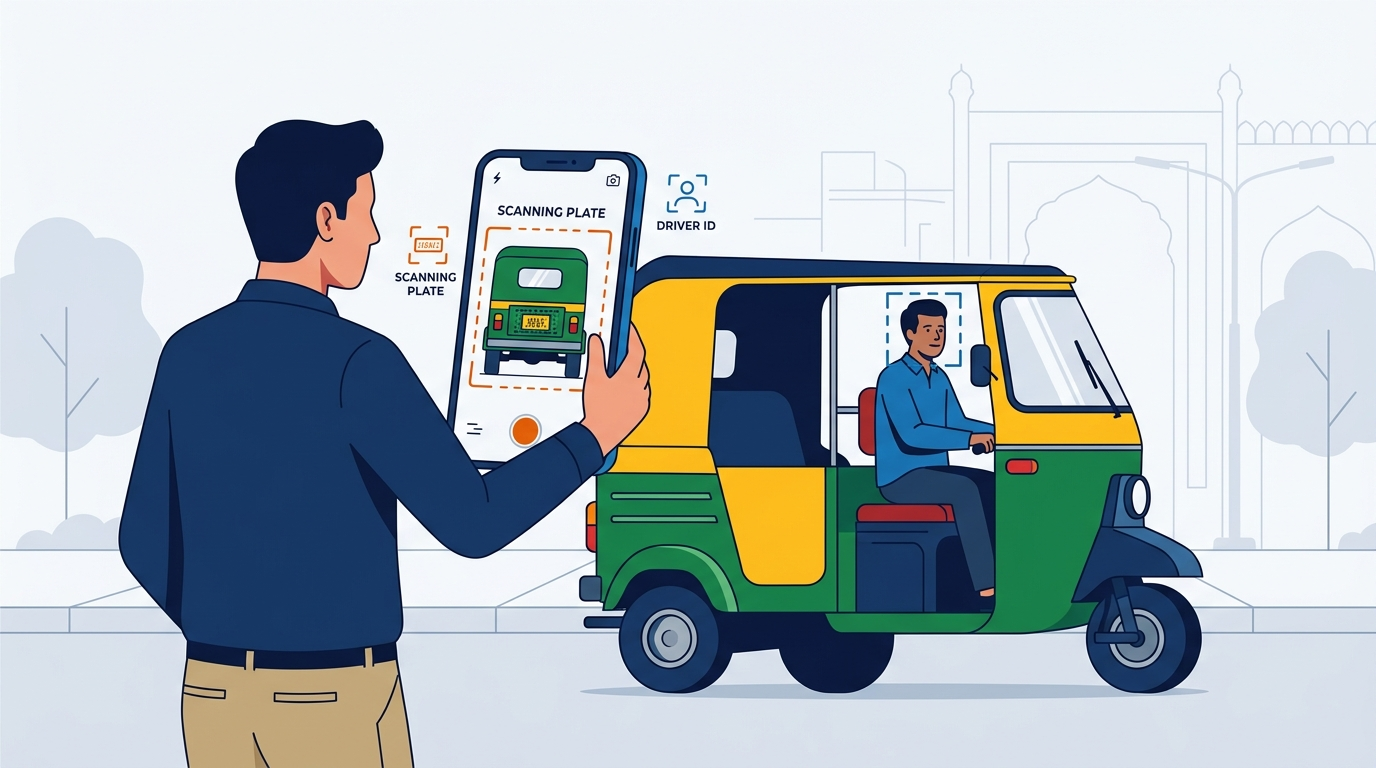
\includegraphics[width=0.86\textwidth]{figures/hero_scan.jpg}
  \caption{The proposed RahiScan interaction. Before boarding, the passenger photographs the rickshaw. The app reads the number plate (orange box) and matches the driver's face (blue box), then returns that driver's history of pace and pricing.}
  \label{fig:hero}
\end{figure}

\textbf{Our proposal.} We propose to build \textbf{RahiScan}, a crowd-sourced mobile app that collects this missing data. A passenger photographs the rickshaw before boarding. The app identifies the vehicle from its Punjab excise number plate and the driver from their face, because many rickshaws are rented by two drivers on different shifts. The passenger types in the quoted fare and starts the ride. From then until arrival the app logs a GPS position every five seconds. After many rides, each driver will have a measured record of how fast they drive compared with the traffic around them, and how their prices compare with a fair benchmark. The next passenger who scans that rickshaw sees the record before agreeing to get in.

The rest of this report takes the story apart stage by stage. For each stage of the Data Science Lifecycle (Lecture 02) we name the problem the story raises, describe how we will handle it, and show what a simulated four-week pilot on \emph{mock data} suggests the result will look like. Every number in this report comes from that simulation, and the dataset and code are in our GitHub repository.

\newpage
% =============================================================================
% 2. LIFECYCLE EXTRACTION
% =============================================================================
\section{Extracting the Data Science Lifecycle from the Story}

The story contains seven separate data science problems, one for each lifecycle stage. Figure~\ref{fig:lifecycle} shows the stages and the guiding question each one answers, and Table~\ref{tab:extract} traces every problem back to the moment in the story that raised it.

\begin{figure}[H]
\centering
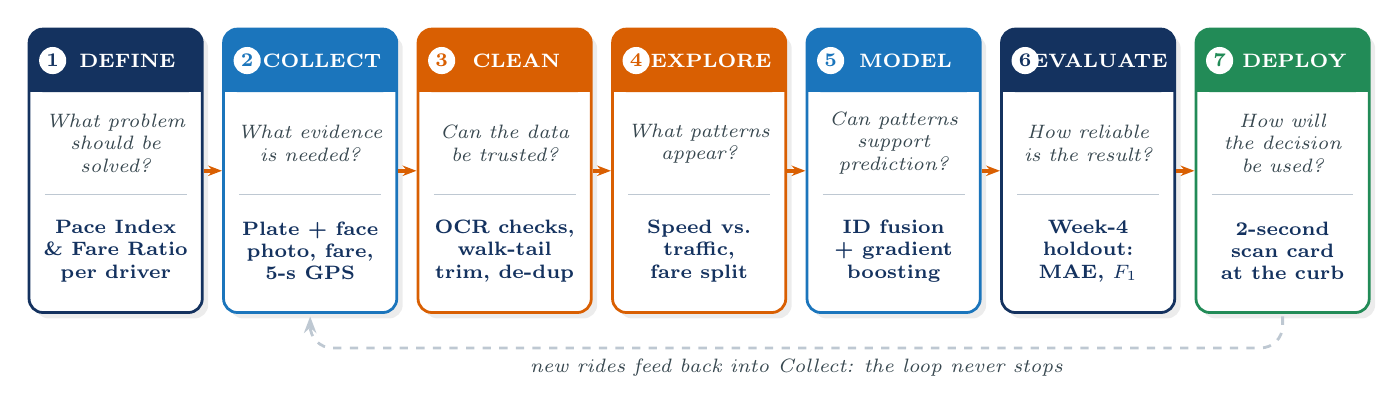
\begin{tikzpicture}[x=1cm, y=1cm]
  \foreach \i/\stage/\q/\act/\col in {
    0/DEFINE/{What problem should be solved?}/{Pace Index \& Fare Ratio per driver}/navyblue,
    1/COLLECT/{What evidence is needed?}/{Plate + face photo, fare, 5-s GPS}/accentblue,
    2/CLEAN/{Can the data be trusted?}/{OCR checks, walk-tail trim, de-dup}/accentorange,
    3/EXPLORE/{What patterns appear?}/{Speed vs. traffic, fare split}/accentorange,
    4/MODEL/{Can patterns support prediction?}/{ID fusion + gradient boosting}/accentblue,
    5/EVALUATE/{How reliable is the result?}/{Week-4 holdout: MAE, \(F_1\)}/navyblue,
    6/DEPLOY/{How will the decision be used?}/{2-second scan card at the curb}/accentgreen%
  }{
    \pgfmathsetmacro{\x}{\i*2.47}
    \draw[rounded corners=5pt, draw=\col, line width=1pt, fill=white, drop shadow={opacity=0.15}] (\x,0) rectangle (\x+2.2,3.6);
    \fill[\col, rounded corners=5pt] (\x,2.8) rectangle (\x+2.2,3.6);
    \fill[\col] (\x,2.8) rectangle (\x+2.2,3.1);
    \node[circle, fill=white, text=\col, font=\bfseries\scriptsize, inner sep=1.2pt] at (\x+0.3,3.2) {\the\numexpr\i+1\relax};
    \node[text=white, font=\bfseries\scriptsize] at (\x+1.25,3.2) {\stage};
    \node[text=slate, font=\itshape\scriptsize, align=center, text width=2.0cm] at (\x+1.1,2.15) {\q};
    \draw[draw=bordergray] (\x+0.2,1.5) -- (\x+2.0,1.5);
    \node[text=navyblue, font=\bfseries\scriptsize, align=center, text width=2.0cm] at (\x+1.1,0.78) {\act};
  }
  \foreach \i in {0,...,5}{
    \draw[-{Stealth[length=5pt]}, line width=1.3pt, draw=accentorange] (\i*2.47+2.22,1.8) -- (\i*2.47+2.45,1.8);
  }
  \draw[-{Stealth[length=6pt]}, line width=1pt, draw=bordergray, dashed, rounded corners=8pt]
     (6*2.47+1.1,-0.05) -- (6*2.47+1.1,-0.45) -- node[below, font=\scriptsize\itshape, text=slate]{new rides feed back into Collect: the loop never stops} (1*2.47+1.1,-0.45) -- (1*2.47+1.1,-0.05);
\end{tikzpicture}
\caption{The seven-stage Data Science Lifecycle applied to RahiScan. Each card pairs the lecture's guiding question with our planned answer.}
\label{fig:lifecycle}
\end{figure}

\begin{table}[H]
\centering\footnotesize
\caption{Data science problems extracted from the case-study story.}
\label{tab:extract}
{\renewcommand{\arraystretch}{1.18}
\begin{tabularx}{\textwidth}{|>{\columncolor{softblue}\bfseries\color{navyblue}}p{1.5cm}|>{\itshape}p{4.6cm}|X|}
\hline
\rowcolor{navyblue}\hdr{Stage} & \hdr{Moment in the story} & \hdr{Data science problem it raises} \\ \hline
Define   & ``We could not tell the two drivers apart.'' & ``Good'' and ``bad'' are vague. We need measurable targets: a speed score that accounts for traffic and a price score against a fair benchmark. \\ \hline
Collect  & ``Every bad ride leaves behind data nobody records.'' & What evidence proves who the driver is, what was charged and how the ride went? We need photos, the fare quote, GPS traces and reference fares. \\ \hline
Clean    & ``We walked into the lab twelve minutes late.'' & Passengers who forget to tap \emph{End Ride} log their walk to class as ride time. Blurry plates, duplicate uploads and fare typos also corrupt the records. \\ \hline
Explore  & ``\ldots even though the traffic was worse.'' & Raw speed blames drivers for traffic jams. Speed has to be compared with what other rickshaws managed on the same road at the same hour. \\ \hline
Model    & ``A different driver took the same route.'' & Identify the right driver, including on shared rickshaws, and predict a fair fare and a pace class from their history. \\ \hline
Evaluate & ``A driver stuck in traffic is not a slow driver.'' & How often would the app wrongly label an honest driver? We need error rates on rides the model has never seen. \\ \hline
Deploy   & ``We had to decide at the curb, in seconds.'' & The answer must reach the passenger as a clear card within two seconds, while protecting driver privacy and allowing appeals. \\ \hline
\end{tabularx}}
\end{table}

\begin{figure}[H]
\centering
\resizebox{\textwidth}{!}{%
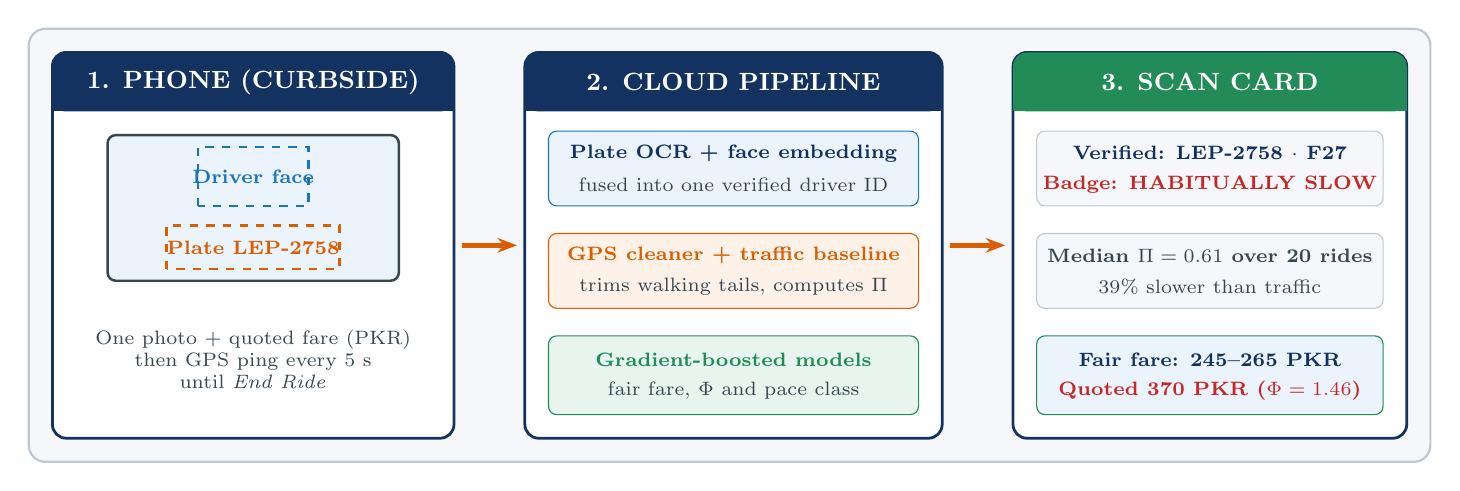
\begin{tikzpicture}
  \draw[rounded corners=6pt, draw=bordergray, line width=0.8pt, fill=lightgray] (0,0) rectangle (17.8,5.5);
  % box 1
  \draw[rounded corners=5pt, draw=navyblue, line width=1pt, fill=white] (0.3,0.3) rectangle (5.4,5.2);
  \fill[navyblue, rounded corners=5pt] (0.3,4.45) rectangle (5.4,5.2); \fill[navyblue] (0.3,4.45) rectangle (5.4,4.75);
  \node[text=white, font=\bfseries\small] at (2.85,4.82) {1. PHONE (CURBSIDE)};
  \draw[rounded corners=3pt, draw=slate, line width=0.9pt, fill=softblue] (1.0,2.3) rectangle (4.7,4.15);
  \draw[dashed, draw=accentblue, line width=1pt] (2.15,3.25) rectangle (3.55,4.0);
  \node[font=\scriptsize\bfseries, text=accentblue] at (2.85,3.62) {Driver face};
  \draw[dashed, draw=accentorange, line width=1pt] (1.75,2.45) rectangle (3.95,3.0);
  \node[font=\scriptsize\bfseries, text=accentorange] at (2.85,2.72) {Plate LEP-2758};
  \node[font=\scriptsize, align=center, text=slate] at (2.85,1.3) {One photo + quoted fare (PKR)\\then GPS ping every 5 s\\until \emph{End Ride}};
  \draw[-{Stealth[length=7pt]}, line width=2pt, draw=accentorange] (5.5,2.75) -- (6.2,2.75);
  % box 2
  \draw[rounded corners=5pt, draw=navyblue, line width=1pt, fill=white] (6.3,0.3) rectangle (11.6,5.2);
  \fill[navyblue, rounded corners=5pt] (6.3,4.45) rectangle (11.6,5.2); \fill[navyblue] (6.3,4.45) rectangle (11.6,4.75);
  \node[text=white, font=\bfseries\small] at (8.95,4.82) {2. CLOUD PIPELINE};
  \draw[rounded corners=3pt, draw=accentblue, fill=softblue] (6.6,3.25) rectangle (11.3,4.2);
  \node[font=\scriptsize\bfseries, text=navyblue] at (8.95,3.92) {Plate OCR + face embedding};
  \node[font=\scriptsize, text=slate] at (8.95,3.52) {fused into one verified driver ID};
  \draw[rounded corners=3pt, draw=accentorange, fill=softorange] (6.6,1.95) rectangle (11.3,2.9);
  \node[font=\scriptsize\bfseries, text=accentorange] at (8.95,2.62) {GPS cleaner + traffic baseline};
  \node[font=\scriptsize, text=slate] at (8.95,2.22) {trims walking tails, computes \(\Pi\)};
  \draw[rounded corners=3pt, draw=accentgreen, fill=softgreen] (6.6,0.6) rectangle (11.3,1.6);
  \node[font=\scriptsize\bfseries, text=accentgreen] at (8.95,1.3) {Gradient-boosted models};
  \node[font=\scriptsize, text=slate] at (8.95,0.9) {fair fare, \(\Phi\) and pace class};
  \draw[-{Stealth[length=7pt]}, line width=2pt, draw=accentorange] (11.7,2.75) -- (12.4,2.75);
  % box 3
  \draw[rounded corners=5pt, draw=navyblue, line width=1pt, fill=white] (12.5,0.3) rectangle (17.5,5.2);
  \fill[accentgreen, rounded corners=5pt] (12.5,4.45) rectangle (17.5,5.2); \fill[accentgreen] (12.5,4.45) rectangle (17.5,4.75);
  \node[text=white, font=\bfseries\small] at (15.0,4.82) {3. SCAN CARD};
  \draw[rounded corners=3pt, draw=bordergray, fill=lightgray] (12.8,3.25) rectangle (17.2,4.2);
  \node[font=\scriptsize\bfseries, text=navyblue] at (15.0,3.92) {Verified: LEP-2758 \(\cdot\) F27};
  \node[font=\scriptsize\bfseries, text=accentred] at (15.0,3.52) {Badge: HABITUALLY SLOW};
  \draw[rounded corners=3pt, draw=bordergray, fill=lightgray] (12.8,1.95) rectangle (17.2,2.9);
  \node[font=\scriptsize\bfseries, text=slate] at (15.0,2.62) {Median \(\Pi = 0.61\) over 20 rides};
  \node[font=\scriptsize, text=slate] at (15.0,2.22) {39\% slower than traffic};
  \draw[rounded corners=3pt, draw=accentgreen, fill=softblue] (12.8,0.6) rectangle (17.2,1.6);
  \node[font=\scriptsize\bfseries, text=navyblue] at (15.0,1.3) {Fair fare: 245--265 PKR};
  \node[font=\scriptsize\bfseries, text=accentred] at (15.0,0.9) {Quoted 370 PKR (\(\Phi = 1.46\))};
\end{tikzpicture}}
\caption{Proposed system architecture. The scan card shows a real driver profile from our mock pilot (driver D27).}
\label{fig:arch}
\end{figure}

% =============================================================================
% 3. DEFINE
% =============================================================================
\section{Define: Turning Frustration into Measurable Targets}
\stagebanner{1}{DEFINE}{What problem should be solved?}{navyblue}

``This driver is slow'' and ``this driver overcharges'' are opinions. To make them testable we define two ratios for every ride \(i\). A value of 1 means typical, so the ratios can be compared across routes and hours.

\begin{tcolorbox}[enhanced, colback=white, colframe=navyblue, boxrule=0.8pt, arc=3pt, sidebyside, sidebyside align=top, lefthand width=0.53\textwidth, left=6pt, right=6pt, top=4pt, bottom=4pt]
{\color{navyblue}\bfseries Driving Pace Index}
\[ \Pi_i = \frac{v_{\mathrm{obs},i}}{v_{\mathrm{base},i}} = \frac{d_i / t_i}{\operatorname{median}(v_{\mathrm{obs}}\text{ on corridor, hour})} \]
{\small A driver at \(\Pi=0.6\) moves 40\% slower than other rickshaws managed on the same road at the same time.}
\tcblower
{\color{accentorange}\bfseries Fare Fairness Ratio}
\[ \Phi_i = \frac{\mathrm{Fare}_{\mathrm{quoted},i}}{\widehat{\mathrm{Fare}}_{\mathrm{fair},i}} \]
{\small \(\widehat{\mathrm{Fare}}_{\mathrm{fair}}\) is predicted from distance, corridor and congestion, using ride-hailing quotes for the same trip as the benchmark.}
\end{tcolorbox}

The app turns these ratios into badges. We fixed the thresholds before looking at any data so they cannot be tuned to flatter the results (Table~\ref{tab:define}). A badge describes a driver's median over at least five rides, never a single ride.

\begin{table}[H]
\centering\small
\caption{Decision rules defined before data collection.}
\label{tab:define}
{\renewcommand{\arraystretch}{1.3}
\begin{tabularx}{\textwidth}{|>{\bfseries}l|c|X|}
\hline
\rowcolor{navyblue}\hdr{Badge} & \hdr{Rule (driver median)} & \hdr{What the passenger is told} \\ \hline
\cellcolor{softred}\textcolor{accentred}{Habitually Slow} & \(\Pi < 0.75\) & Expect a ride at least 25\% longer than traffic requires. \\ \hline
\cellcolor{softgreen}\textcolor{accentgreen}{Normal Pace} & \(0.75 \le \Pi \le 1.15\) & Moves with traffic. \\ \hline
\cellcolor{softblue}\textcolor{accentblue}{Fast} & \(\Pi > 1.15\) & Noticeably quicker than traffic. \\ \hline
\cellcolor{softorange}\textcolor{accentorange}{Overpriced} & \(\Phi > 1.25\) & Usually quotes more than 25\% above the fair fare. Negotiate. \\ \hline
\end{tabularx}}
\end{table}

% =============================================================================
% 4. COLLECT
% =============================================================================
\section{Collect: The Evidence We Need}
\stagebanner{2}{COLLECT}{What evidence is needed?}{accentblue}

No public dataset links a Lahore rickshaw driver to their speed and prices, so RahiScan will collect its own. We plan a four-week pilot with about 85 student volunteers on eight commuter corridors around campus. Table~\ref{tab:collect} lists the five data streams. We designed each one around a question the later stages must answer.

\begin{table}[H]
\centering\small
\caption{Planned data streams and the volume produced by our simulated pilot.}
\label{tab:collect}
{\renewcommand{\arraystretch}{1.3}
\begin{tabularx}{\textwidth}{|>{\columncolor{softblue}\bfseries}p{2.6cm}|X|p{2.5cm}|>{\raggedleft\arraybackslash}p{2.0cm}|}
\hline
\rowcolor{navyblue}\hdr{Stream} & \hdr{Fields captured} & \hdr{Why we need it} & \hdr{Mock rows} \\ \hline
Curb scan     & Plate OCR text and confidence, face-embedding match and similarity, low-light flag & Who is driving? & 1,200 \\ \hline
Ride record   & User, corridor, start and end time, quoted fare (PKR), \emph{End Ride} tapped? & What was charged? & 1,224 \\ \hline
GPS pings     & Latitude, longitude, timestamp every 5 s, accelerometer step variance & How was the ride driven? & 364,488 \\ \hline
Fare benchmark & inDrive, Careem or Bykea quote for the same origin and destination & What is a fair fare? & 1,200 \\ \hline
Driver gallery & Plate to driver(s), face ID, shift (34 vehicles, 40 drivers) & Who shares a rickshaw? & 40 \\ \hline
\end{tabularx}}
\end{table}

\begin{figure}[H]
  \centering
  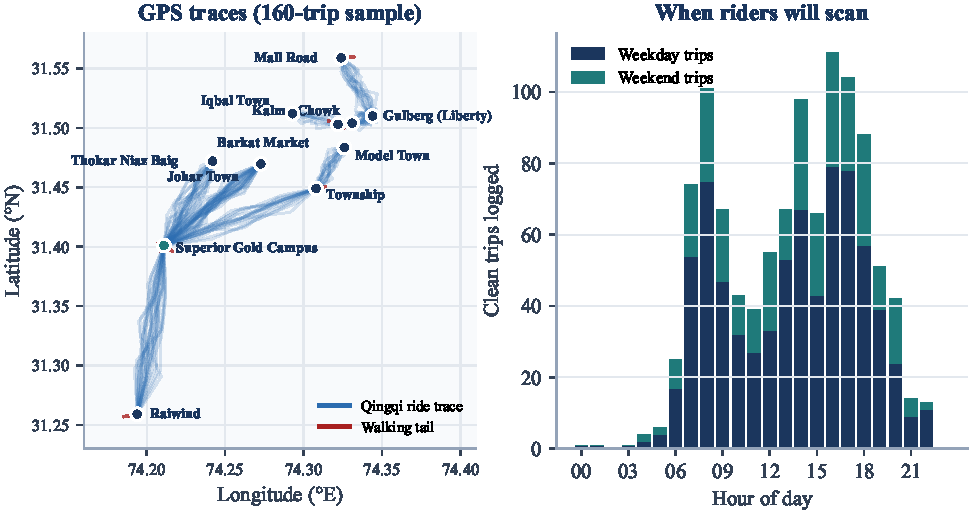
\includegraphics[width=\textwidth]{figures/fig_route_map.pdf}
  \caption{Left: simulated GPS traces on the eight pilot corridors, with walking tails from forgotten \emph{End Ride} taps in red. Right: trips cluster in the morning and evening rush, which is exactly when traffic and driver behaviour are hardest to separate.}
  \label{fig:collect}
\end{figure}

\textbf{Consent and privacy.} Face data is sensitive. Drivers will be told about the pilot and may opt out. The app will store only a numeric face embedding, never the photo itself, and pings recorded before boarding or after the ride ends will be deleted once cleaning is complete.

% =============================================================================
% 5. CLEAN
% =============================================================================
\section{Clean: Can the Data Be Trusted?}
\stagebanner{3}{CLEAN}{Can the data be trusted?}{accentorange}

Crowd-sourced data from phones on a busy street will be messy, so we put realistic faults into the mock data on purpose and wrote one rule for each. \textbf{Duplicate uploads} caused by weak mobile signal are dropped when the same user submits the same corridor within ten seconds. \textbf{Fare errors}, either blank or with an extra zero typed in (5,200 instead of 520), are removed when the quote is more than four times or less than 0.4 times the benchmark. \textbf{Identity errors} come from dented or glared plates at night. We accept a plate read only when OCR confidence is at least 0.85. Otherwise the face match must reach a similarity of 0.70, and when two drivers share a plate the face decides between them. Rides with less than 75\% \textbf{GPS coverage}, usually from underpasses, are excluded. Figure~\ref{fig:clean} shows how many records each rule removes, and shows that adding the face check raises identification precision from 85.7\% to 99.8\%.

\begin{figure}[H]
  \centering
  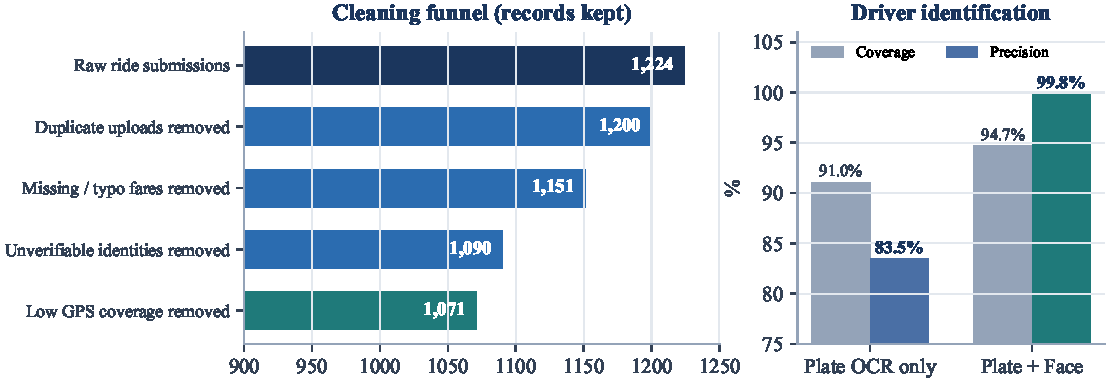
\includegraphics[width=\textwidth]{figures/fig_cleaning.pdf}
  \caption{Left: 1,224 raw submissions shrink to 1,058 trusted rides. Right: fusing face and plate both identifies more rides (coverage) and makes fewer mistakes (precision) than reading the plate alone.}
  \label{fig:clean}
\end{figure}

The most damaging fault is the \textbf{walking tail} from our own story. A student who jumps out and forgets to tap \emph{End Ride} keeps recording a slow walk into the building, which pulls the driver's average speed down. Our filter works back from the end of the trace and cuts every ping where speed stays under 6\,km/h \emph{and} the accelerometer shows walking steps for at least a minute. On the mock data it caught 88\% of the 130 tails with no false cuts, and it restored a median of 3.1\,km/h to each affected driver's speed (Figure~\ref{fig:trim}). Most of the tails it missed had very weak step signals, which matches a phone carried in a bag.

\begin{figure}[H]
  \centering
  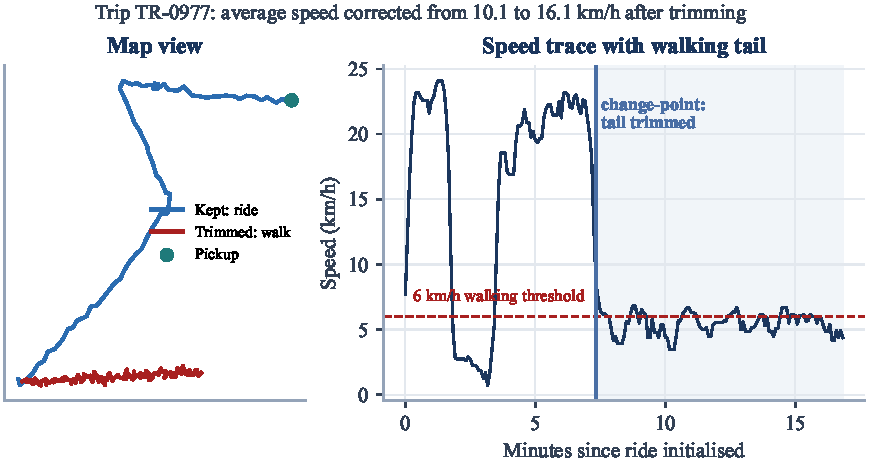
\includegraphics[width=\textwidth]{figures/fig_gps_trim.pdf}
  \caption{Change-point trimming on one simulated ride. Without the trim, an honest driver would have looked 28\% slower than they were.}
  \label{fig:trim}
\end{figure}

% =============================================================================
% 6. EXPLORE
% =============================================================================
\section{Explore: What Patterns Appear?}
\stagebanner{4}{EXPLORE}{What patterns appear?}{accentorange}

The first thing to look at is traffic. Figure~\ref{fig:heat} shows the crowd-sourced baseline speed \(v_{\mathrm{base}}\), the median over all drivers, for each corridor and two-hour window. On Mall Road the baseline drops from 22\,km/h at night to 5\,km/h at 4 pm. A driver doing 7\,km/h at that hour is keeping up with traffic. The same speed at 10 pm would be very slow. Raw speed alone cannot tell these cases apart, which is why \(\Pi\) is defined against the baseline.

\begin{figure}[H]
  \centering
  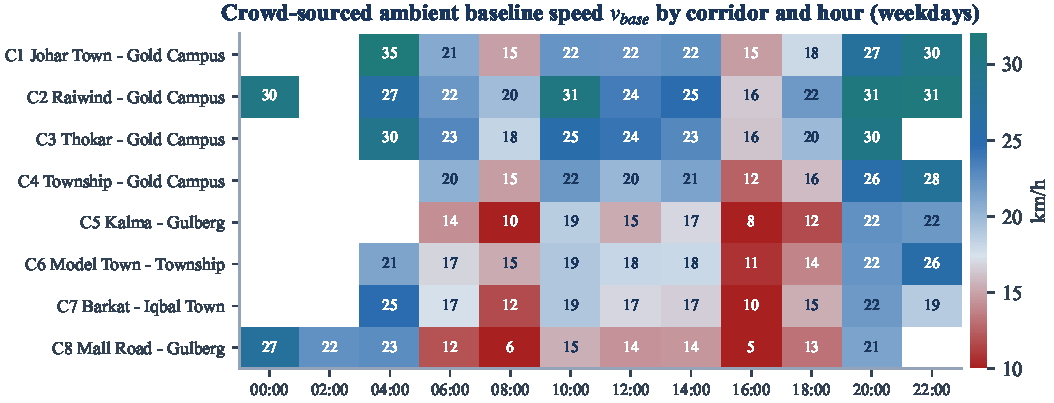
\includegraphics[width=\textwidth]{figures/fig_heatmap.pdf}
  \caption{Median ambient speed by corridor and hour on weekdays (mock pilot). Red cells are rush-hour bottlenecks where raw speed would unfairly penalise drivers.}
  \label{fig:heat}
\end{figure}

\begin{figure}[H]
  \centering
  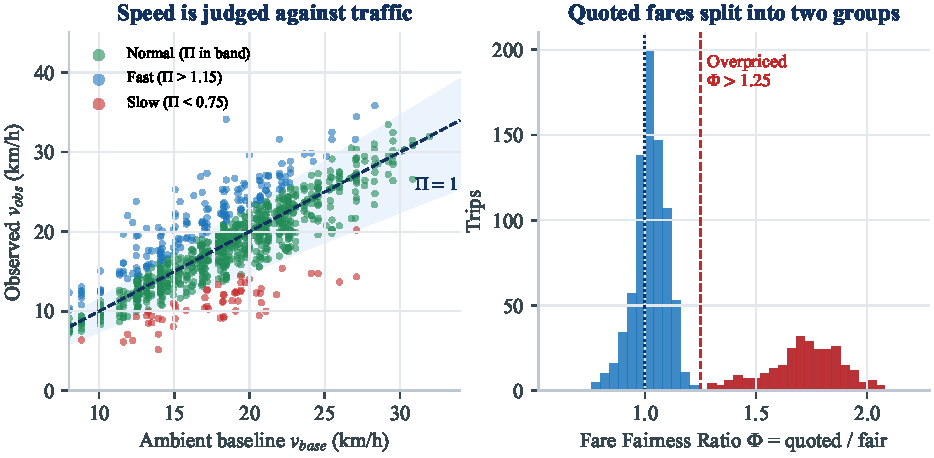
\includegraphics[width=\textwidth]{figures/fig_explore.pdf}
  \caption{Left: each dot is one ride. Rides inside the blue band move with traffic regardless of absolute speed. Right: the Fare Ratio splits into a fair cluster near 1.0 and an overpriced cluster near 1.7.}
  \label{fig:explore}
\end{figure}

Table~\ref{tab:sample} shows six cleaned rides. Ride TR-0827 moved at only 7.3\,km/h, yet \(\Pi=0.91\) because Kalma Chowk was gridlocked at 5 pm, so that driver is not penalised. Ride TR-0597 was slower than traffic \emph{and} quoted 46\% above the fair fare. TR-0266 shows a driver who keeps pace but asked for twice the fair fare, and the two scores capture these as separate problems.

\begin{table}[H]
\centering\footnotesize
\caption{Sample of the cleaned, feature-engineered mock dataset (\texttt{data/processed/trips\_clean.csv}).}
\label{tab:sample}
{\renewcommand{\arraystretch}{1.3}\setlength{\tabcolsep}{4pt}
\begin{tabular}{|>{\columncolor{softblue}\bfseries}c|c|l|c|c|c|c|c|c|c|}
\hline
\rowcolor{navyblue}\hdr{Ride} & \hdr{Plate \# Face} & \hdr{Corridor} & \hdr{Hour} & \hdr{km} & \hdr{\(v_{\mathrm{obs}}\)} & \hdr{\(v_{\mathrm{base}}\)} & \hdr{\(\Pi\)} & \hdr{Quoted / Fair} & \hdr{\(\Phi\)} \\ \hline
TR-0466 & \texttt{LEP-4334\#F04} & Thokar -- Campus & 14 & 8.5 & 25.6 & 24.6 & 1.04 & 460 / 458 & \textcolor{accentgreen}{\textbf{1.00}} \\ \hline
TR-0824 & \texttt{LER-5034\#F17} & Johar Town -- Campus & 11 & 9.9 & 29.1 & 25.5 & 1.14 & 500 / 519 & \textcolor{accentgreen}{\textbf{0.96}} \\ \hline
TR-0827 & \texttt{LEP-4877\#F22} & Kalma -- Gulberg & 17 & 2.1 & 7.3 & 8.0 & \textcolor{accentgreen}{\textbf{0.91}} & 180 / 169 & \textcolor{accentgreen}{\textbf{1.07}} \\ \hline
TR-0597 & \texttt{LEP-2758\#F27} & Barkat -- Iqbal Town & 8 & 3.9 & 6.1 & 11.6 & \textcolor{accentred}{\textbf{0.53}} & 370 / 254 & \textcolor{accentred}{\textbf{1.46}} \\ \hline
TR-0266 & \texttt{LES-8870\#F32} & Township -- Campus & 7 & 10.8 & 17.4 & 18.2 & 0.96 & 1070 / 528 & \textcolor{accentred}{\textbf{2.03}} \\ \hline
TR-0252 & \texttt{LEB-5028\#F25} & Johar Town -- Campus & 17 & 10.1 & 17.7 & 14.1 & \textcolor{accentblue}{\textbf{1.26}} & 510 / 557 & \textcolor{accentgreen}{\textbf{0.92}} \\ \hline
\end{tabular}}
\end{table}

% =============================================================================
% 7. MODEL
% =============================================================================
\section{Model: From Patterns to Predictions}
\stagebanner{5}{MODEL}{Can patterns support prediction?}{accentblue}

The modelling plan has two tiers (Figure~\ref{fig:journey}). \textbf{Tier 1, identity:} a lightweight MobileNetV3 face encoder and a plate OCR model produce two candidate IDs, and the fusion rule from the Clean stage combines them into one verified driver. This tier matters because in our mock gallery six rickshaws are shared between a day driver and an evening driver. Plate \texttt{LES-8113}, for example, belongs to a fair day driver (\(\Phi=1.05\)) and an overpriced evening driver (\(\Phi=1.77\)), and a plate-only system would average the two into one misleading score. \textbf{Tier 2, behaviour:} a gradient-boosted regressor predicts the fair fare from distance, corridor, hour, day type and \(v_{\mathrm{base}}\). A gradient-boosted classifier predicts each ride's pace class, and the driver's badge is the median over their history.

\begin{figure}[H]
  \centering
  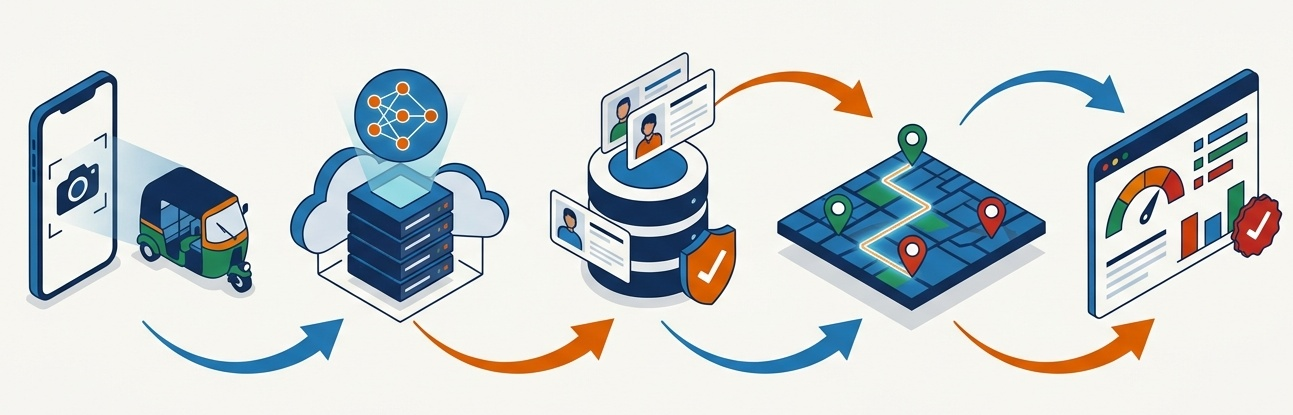
\includegraphics[width=0.86\textwidth]{figures/data_journey.jpg}
  \caption{Data journey of a single scan: phone photo, cloud identity models, driver profile database, GPS ride trace, and the scorecard returned to the passenger.}
  \label{fig:journey}
\end{figure}

Figure~\ref{fig:quadrant} plots every simulated driver's profile after four weeks. Most drivers sit in the fair, normal-pace corner. Eleven form an overpriced cluster, three are habitually slow, and two (\texttt{LEP-2758} and \texttt{LES-8176}) are both slow and overpriced. That pair is the kind of driver from our first morning.

\begin{figure}[H]
  \centering
  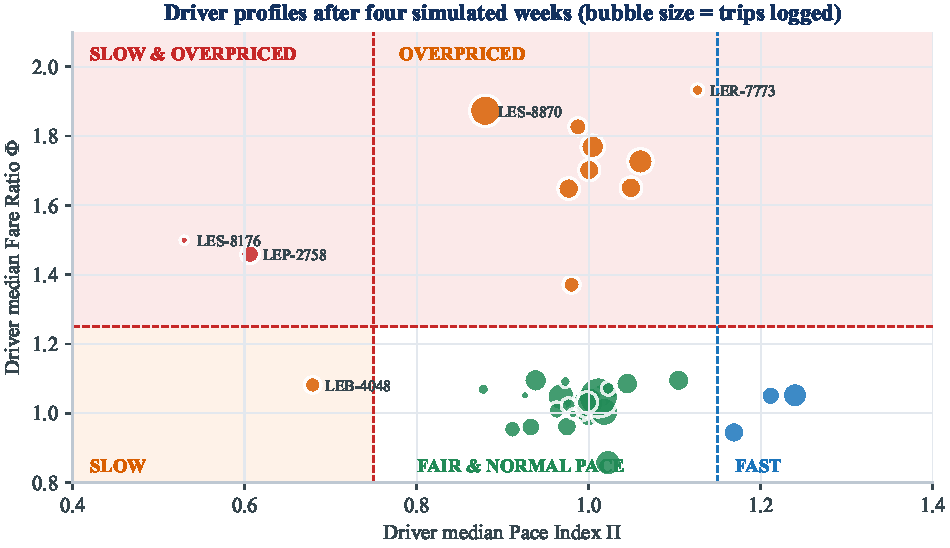
\includegraphics[width=0.90\textwidth]{figures/fig_quadrant.pdf}
  \caption{Driver-level profiles in the mock pilot. The two axes are independent: pricing and pace are separate behaviours and need separate badges.}
  \label{fig:quadrant}
\end{figure}

% =============================================================================
% 8. EVALUATE
% =============================================================================
\section{Evaluate: How Reliable Is the Result?}
\stagebanner{6}{EVALUATE}{How reliable is the result?}{navyblue}

We will train on weeks 1 to 3 and test on week 4 only, so every reported score comes from rides the models have never seen, in time order as they would occur in real use. Each module also has a simpler baseline to beat. Table~\ref{tab:eval} compares the targets we set in advance with the mock-pilot results.

\begin{table}[H]
\centering\footnotesize
\caption{Evaluation targets versus simulated results on the week-4 holdout (280 rides, 40 drivers).}
\label{tab:eval}
{\renewcommand{\arraystretch}{1.18}
\begin{tabularx}{\textwidth}{|>{\columncolor{softblue}\bfseries}p{2.7cm}|X|>{\centering\arraybackslash}p{1.6cm}|>{\centering\arraybackslash}p{2.4cm}|>{\centering\arraybackslash}p{1.5cm}|}
\hline
\rowcolor{navyblue}\hdr{Module} & \hdr{Metric (baseline)} & \hdr{Target} & \hdr{Mock result} & \hdr{Status} \\ \hline
Driver identity & Precision of verified IDs (plate only: 85.7\%) & \(\ge 93\%\) & \textbf{99.8\%} & \cellcolor{softgreen}\textcolor{accentgreen}{\textbf{Met}} \\ \hline
Walking-tail filter & Recall of forgotten \emph{End Ride} taps & \(\ge 0.85\) & \textbf{0.88} & \cellcolor{softgreen}\textcolor{accentgreen}{\textbf{Met}} \\ \hline
Fair-fare regressor & Mean absolute error (linear: 12.1, flat rate: 117.6 PKR) & \(< 15\) PKR & \textbf{10.9 PKR} & \cellcolor{softgreen}\textcolor{accentgreen}{\textbf{Met}} \\ \hline
Pace, single ride & Macro \(F_1\) (raw speed only: 0.45) & \(\ge 0.88\) & \textbf{0.67} & \cellcolor{softred}\textcolor{accentred}{\textbf{Not met}} \\ \hline
Pace, driver badge & Accuracy over \(\ge 5\) rides (raw speed only: 87.5\%) & \(\ge 90\%\) & \textbf{100\%} & \cellcolor{softgreen}\textcolor{accentgreen}{\textbf{Met}} \\ \hline
Fare badge & Accuracy of the Overpriced flag & \(\ge 90\%\) & \textbf{100\%} & \cellcolor{softgreen}\textcolor{accentgreen}{\textbf{Met}} \\ \hline
\end{tabularx}}
\end{table}

\begin{figure}[H]
  \centering
  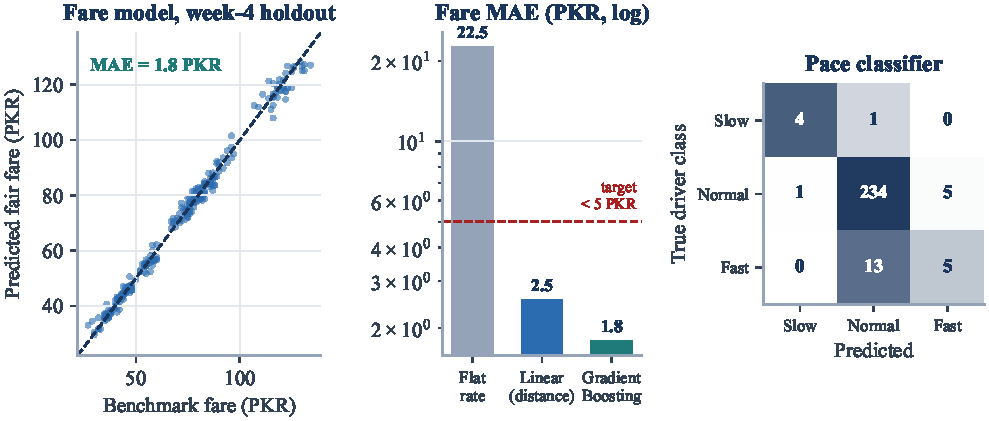
\includegraphics[width=0.92\textwidth]{figures/fig_evaluate.pdf}
  \caption{Holdout evaluation. Left and centre: the fare model beats both baselines and stays under the 15 PKR target. Right: single-ride pace predictions mostly confuse Fast and Slow drivers with Normal ones.}
  \label{fig:eval}
\end{figure}

The single-ride pace classifier is the one result that misses its target, and the miss changes how we will deploy. One ride is noisy: a slow driver can catch every green light, and a fast driver can sit behind a broken-down bus. Over several rides the median settles, and driver-level badge accuracy reaches 100\%, against 87.5\% when speed is not compared with traffic (Figure~\ref{fig:norm}). The app will therefore never label a driver from one ride. It will show \emph{Not enough data} until five rides have been logged.

\begin{figure}[H]
  \centering
  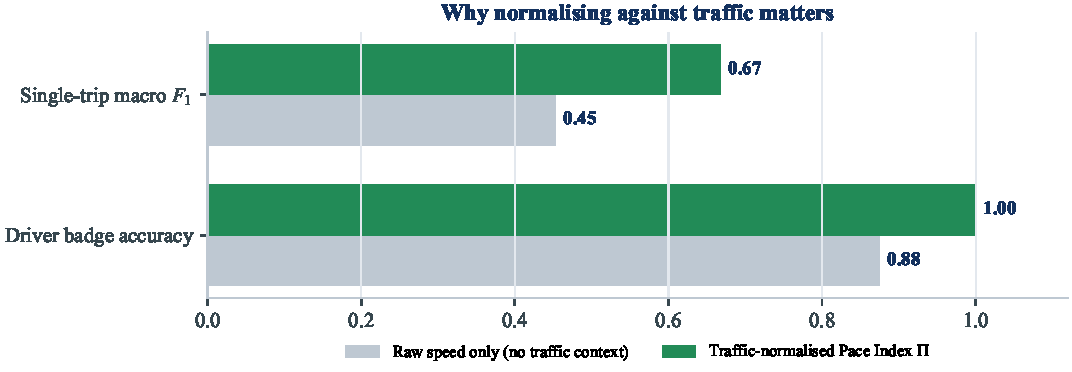
\includegraphics[width=0.86\textwidth]{figures/fig_normalisation.pdf}
  \caption{Normalising speed against the crowd-sourced traffic baseline improves results for both single rides and driver badges.}
  \label{fig:norm}
\end{figure}

% =============================================================================
% 9. DEPLOY
% =============================================================================
\newpage
\section{Deploy: How Will the Decision Be Used?}
\stagebanner{7}{DEPLOY}{How will the decision be used?}{accentgreen}

The evaluated models will run behind a lightweight cloud API. The passenger's experience has three screens (Figure~\ref{fig:app}): scan the rickshaw, ride with live tracking, and read a card showing the driver's verified identity, pace badge, and fair-fare range next to the quote. Our target is to return the card within two seconds of the photo. That leaves time to negotiate, or to wave the rickshaw on and wait for the next one, before the driver pulls away.

\begin{figure}[H]
  \centering
  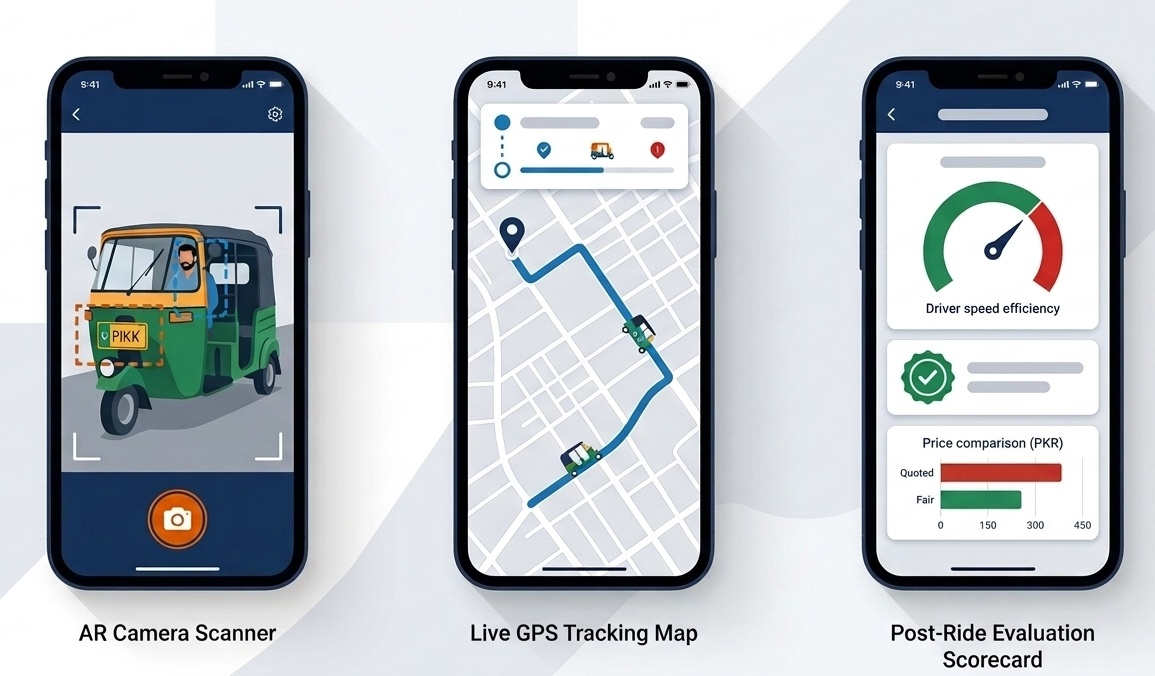
\includegraphics[width=0.50\textwidth]{figures/app_mockup.jpg}
  \caption{Proposed app flow: AR scan at the curb, live GPS ride tracking, and the post-scan scorecard with pace gauge and quoted-versus-fair price bars.}
  \label{fig:app}
\end{figure}

Deployment also adds safeguards that a classroom model does not need. Drivers will be able to view and dispute their own profile, and a badge appears only after five verified rides. Profiles will weight recent rides more heavily, so a driver who improves is not held back by old data. Because fuel prices change, the fare model will be retrained every month against fresh ride-hailing benchmarks. Every new ride flows back into the Collect stage, which closes the loop shown in Figure~\ref{fig:lifecycle}. Figure~\ref{fig:timeline} shows the eight-week plan from prototype to campus beta.

\begin{figure}[H]
  \centering
  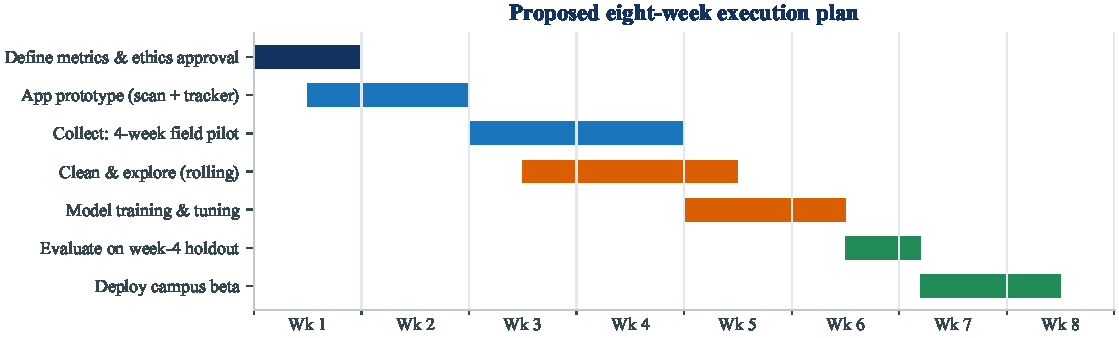
\includegraphics[width=0.68\textwidth]{figures/fig_timeline.pdf}
  \caption{Proposed execution timeline. The four-week field pilot supplies the data for every later stage.}
  \label{fig:timeline}
\end{figure}

\begin{insight}[Conclusion]
Our rickshaw story contained a problem for every stage of the lifecycle. The simulated pilot suggests that RahiScan can identify drivers reliably by combining plate and face, and that it can price fares to within about 11 rupees. It also suggests that drivers can be judged fairly on pace only when speed is compared with traffic and averaged over several rides. With real rides in place of mock ones, the same pipeline in our repository would give Lahore's student commuters the information they currently lack at the curb.
\end{insight}

\end{document}
